\documentclass[8pt]{beamer}

\usepackage[utf8]{inputenc}
\usepackage{lmodern}
\usepackage{beamerthemesplit} 
\usepackage{pstricks}
\usepackage{pst-node}
\usepackage{graphicx}



\newcommand{\E}{\mathbb{E}}
\newcommand{\Proba}{\mathbb{P}}
\newcommand{\F}{\mathcal{F}}
\newcommand{\Bt}{B_t}
\newcommand{\DtT}{D(t,T)}
\newcommand{\RtT}{R(t,T)}
\newcommand{\PtT}{P(t,T)}
\newcommand{\PtS}{P(t,S)}
\newcommand{\LtT}{l(t,T)}
\newcommand{\YtT}{Y(t,T)}
\newcommand{\ftT}{f(t,T)}
\newcommand{\tautT}{\tau(t,T)}
\newcommand{\inttT}{\int_t^T}
\newcommand{\intt}{\int_0^t}
\newcommand{\FuncExp}{\text{exp}}
\newcommand{\FuncLn}{\text{ln}}
\newcommand{\Discount}[2]{e^{-\int_{#1}^{#2}r_u du} }
\newcommand{\bl}[1]{{\scshape  #1}}

\newcommand{\Ti}{T_{i}}
\newcommand{\Tj}{T_{j}}
\newcommand{\Ta}{T_{\alpha}}
\newcommand{\Tb}{T_{\beta}}
\newcommand{\Tii}{T_{i+1}}
\newcommand{\Pti}{P(t,T_{i})}
\newcommand{\Ptii}{P(t,T_{i+1})}
\newcommand{\Lti}{L(t,\Ti,\Tii)}
\newcommand{\Lit}{L_{i}(t)}
\newcommand{\muit}{\mu_i(t)}
\newcommand{\sigmait}{\sigma_i(t)}
\newcommand{\Wit}{W^{\Tii}(t)}
\newcommand{\Wnt}{W^{T_{N+1}}(t)}
\newcommand{\Ltj}{L(t,\Tj,\Tj)}
\newcommand{\Ljt}{L_{j}(t)}
\newcommand{\sigmajt}{\sigma_j(t)}
\newcommand{\ZCi}{ZC_{i}}
\newcommand{\ZCii}{ZC_{i+1}}
\newcommand{\Numi}{Num_{i}}
\newcommand{\Numii}{Num_{i+1}}

\newcommand{\Sab}{S_{\alpha,\beta}}
\newcommand{\Cab}{C_{\alpha,\beta}}
\newcommand{\Wab}{W_{\alpha,\beta}}
\newcommand{\sigmaab}{\sigma_{\alpha,\beta}}
\newcommand{\rhoij}{\rho_{ij}}
\newcommand{\Eab}{\mathbb{E}^{\alpha,\beta}}




\title[Off-Cycle internship]{Internship Lunalogic M2MO}
\author[Chi Thanh NGUYEN]{NGUYEN Chi Thanh}
\institute[Lunalogic - M2MO]{Lunalogic and M2MO}
\date{2014}

\begin{document}

\begin{frame}[plain]
\titlepage
\end{frame}

\begin{frame}
\tableofcontents
\end{frame}

%%%%%%%%%%%%%%%%%%%%%%%%%%%%%%%%%%%%%%%%%%%%%%%%%%%%%%%%%%%%%%%%
\section{Introduction}
%%%%%%%%%%%%%%%%%%%%%%%%%%%%%%%%
\begin{frame}
\frametitle{Internship concern}
Basical fixed income instruments 
\begin{itemize}
	\item Bond, FRA, Swap rate
	\item Yield Curve, discount rate curve
\end{itemize}
Two famillies plain vanilla derivative
\begin{itemize}
	\item Caplet, Flooret, Caps/Floors
	\item Swaption
	\item Implied Volatility and Black formula
\end{itemize}
Calibration LMM volatility
\begin{itemize}
	\item calibration with caplet quotes, swaption quotes, VCUB
	\item Link LMM Vol , Swaption Vol, Rebonato formula
	\item Calibration Algorithm, test and result
\end{itemize}
\end{frame}


%%%%%%%%%%%%%%%%%%%%%%%%%%%%%%%%
\begin{frame}
\frametitle{Bond, Forward Rate, Swap rate}
Link Bond and Forward Rate
\[
L_i(t) = L(t,\Ti,\Tii) = \frac{1}{\tau_i} \left[ \frac{\Pti}{\Ptii} - 1  \right]
\hspace{1cm}
{\Ptii} = \frac{\Pti}{1+ \tau_i L_i(t)}
\]
Swap Rate can see as weighted sum of Libors
\[
S_{\alpha,\beta}(t) 
= 
\frac{P(t,T_{\alpha})-P(t,T_{\beta})}{\sum^{\hat{\beta}-}_{\hat{i}=\hat{\alpha}}\tau_{\hat{i}}P(t,T_{\hat{i}++})} 
=
\frac{\sum^{\beta-1}_{i=\alpha} \tau_i \Ptii }{\Cab(t)} \Lit
\]
Libor and Swap can be considered as a basket of tradable instruments
\end{frame}

%%%%%%%%%%%%%%%%%%%%%%%%%%%%%%%%
\begin{frame}
\frametitle{Numeraire change and Black Formula - Caplet}
Caplet Payoff at Maturity
\[
\text{price}(T_1) = \tau(T_1,T_2)( L(T_1;T_1,T_2) - K )^+ 
\]
Numeraire change to $P(t,T_2)$ price formula at time zero
\[
\text{price}(0) = \tau(T_1,T_2)P(0,T_2) \mathbb{E}^{T_2}\left[ ( L(T_1;T_1,T_2) - K )^+  \right]
\]
Libor dynamic
\[
\frac{dL(t;T_1,T_2)}{L(t;T_1,T_2)} = \sigma_{L}(t)dW^{T_2}_t
\hspace{2cm}
t\leq T_1 < T_2
\]
Black Formula
\end{frame}

%%%%%%%%%%%%%%%%%%%%%%%%%%%%%%%%
\begin{frame}
\frametitle{Numeraire change and Black Formula - Swaption}
Swaption Payoff at Maturity
\[
\text{price}(\Ta) = \left[ \Sab(\Ta) - K \right]^+ \Cab(\Ta)
\hspace{1cm}
\Cab(t) = \sum^{\beta-1}_{\alpha} \tau_i \Ptii 
\] 
Numeraire change to $\Cab(t)$ price formula at time zero
\[
\text{price}(0) = \Cab(0) \Eab \left[ (\Sab(\Ta) - K )^+  \right]
\]
Swap rate dynamic
\[
\frac{d\Sab(t)}{\Sab(t)} = \sigmaab(t) d\Wab(t)
\]
\begin{itemize}
\item Black Formula
\item Incompatibility with Caplet case
\end{itemize}
\end{frame}

%%%%%%%%%%%%%%%%%%%%%%%%%%%%%%%%%%%%%%%%%%%%%%%%%%%%%%%%%%%%%%%%
\section{LMM Model and Components}
%%%%%%%%%%%%%%%%%%%%%%%%%%%%%%%%
\begin{frame}
\frametitle{Libor Model Setting}
Lognormal Forward rate model under zero coupon numeraire
\[
\frac{d\Lit}{\Lit} = \sigmait d\Wit 
\hspace{1cm}
d\Wit d\Wit = \hat{\rho} dt
\]
Timeline setting , Fixed Float Tenor different. Example for European market 
\[
T_i , i = 0,1, .... N+1. 
\hspace{1cm}
T_0=0,
\hspace{1cm}
T_N=\text{horizon}
\]
Matrix Format are all (N+1)x(N+1)
\end{frame}

%%%%%%%%%%%%%%%%%%%%%%%%%%%%%%%%
\begin{frame}
\frametitle{Libor Model Setting - Matrix Format}
\begin{figure}[h]
\begin{center}
\psset{unit=0.8cm}
\begin{pspicture}(-7,-3)(7,4)
%% Reference for Picture
%\psline[linewidth=0.1pt,linecolor=gray](-7,-3)(7,4)
%\rput(-2,-2){(-2,-2)}\rput(3,3){(3,3)}\rput(0,0){(0,0)}
%%%%%%%%%%%%%%%%%%%%%%%%%%%%%%%%%%%%%%%%%%%%%%%%%%%%%%%%%%%%%%%%%%%%
%% Draw libor matrix
\psgrid[gridwidth=0.01pt,gridcolor=lightgray,subgriddiv=2,subgridwidth=0.1pt,subgridcolor=lightgray,gridlabels=0](-2,-2)(3,3)          % set grid for vol matrix
%% set horizon label for vol matrix
\rput(-2,3.1){$\scriptstyle{T_0}$}
\rput(-1.5,3.1){$\scriptstyle{T_1}$}
\rput(0,3.1){$\scriptstyle{\Tj}$}
\rput(3,3.1){$\scriptstyle{T_{N}}$} 
%% set vertical label for vol matrix
\rput(-2.5,2.5){$L_{1}(.)$}
\rput(-2.5,2){$L_{2}(.)$}
\rput(-2.5,0){$L_i(.)$}
\rput(-2.5,-2){$L_{N}(.)$}     
\rput(0,0){$\bullet$}\rput(0.5,0.2){$L_{i}(\Tj)$}
%%
%%%%%% draw the lower triangular part of libor matrix
{
\pspolygon[fillstyle=crosshatch,hatchcolor=gray,hatchwidth=0.1pt,hatchsep=1pt,linestyle=none](-2,3)(-2,-2)(3,-2)
}
%%%%%% draw the volatility zone
{
\pspolygon[linearc=0.1,linecolor=blue](-1.6,2.8)(3.3,-2.1)(-1.6,-2.1)
}
\end{pspicture}
\end{center}
\caption{\label{fig:libor_matrix} Lower triangular matrix storing Libor values. Volatilities use the same matrix format, but values used are only in blue zone}
\end{figure}
\end{frame}


%%%%%%%%%%%%%%%%%%%%%%%%%%%%%%%%
\begin{frame}
\frametitle{Libor dynamic and translated Brownian}
Numeraire change from $\Pti$ to $\Ptii$
\[
\frac{dQ^{\Tii}}{dQ^{\Ti}} = \frac{P(0,\Tii)}{P(0,\Ti)}\frac{\Pti}{\Ptii} = \textbf{c} (\tau_i \Lit + 1 )
\]
Dynamic $\Lit$ under $Q^{\Tii}$
\[
\frac{d (\textbf{c} (\tau_i \Lit + 1 )) }{\textbf{c} (\tau_i \Lit + 1 )} 
= \frac{\tau_i d\Lit }{\tau_i \Lit +1} = \frac{\tau_i \Lit s_i(t) \hat{\rho}^{\frac{1}{2} }  }{\tau_i \Lit +1} dW^{\Tii} = \mu(t)dW^{\Tii}
\]
Solution is a geometric Brownian, apply Girsanov to the first equation we have the translated Brownian
\[
dW^{T_{k}} = dW^{T_{k+1}} - \frac{\tau_k L_k(t)}{\tau_k L_k(t) +1}  s_k(t) \hat{\rho}^{\frac{1}{2} }_k  dt
\]
Libor dynamic under terminal measure
\[
\frac{d\Lit}{\Lit} = \muit + \sigmait \hat{\rho}^{\frac{1}{2} } dW(t)
\hspace{1cm}
\muit = \sum_{k=i+1}^{N+1} \frac{\tau_j \Ljt}{1+\tau_j \Ljt} \sigmait \sigmajt \hat{\rho}_{ij}
\]
\end{frame}

%%%%%%%%%%%%%%%%%%%%%%%%%%%%%%%%
\begin{frame}
\frametitle{Correlation - Decorrelation}
Parameterized correlation
\[
\hat{\rho}_{ij} = e^{- \beta \frac{ |i-j| }{(i+j)^{\alpha}}}
\]
Singular Value Decomposition
\[
\hat{\rho}_{ij} = PDP^t \hspace{2cm} \rho = \tilde{P}\tilde{D}\tilde{P}^t
\]
Approximation Correlation, reduced factors
\[
\rho^{\frac{1}{2}} =  \tilde{P}\tilde{D}^{\frac{1}{2}}
\]
Libor dynamic with reduced correlation
\[
\frac{d\Lit}{\Lit} = \muit + \sigmait \rho^{\frac{1}{2} } dW(t)
\hspace{1cm}
\muit = \sum_{k=i+1}^{N+1} \frac{\tau_j \Ljt}{1+\tau_j \Ljt} \sigmait \sigmajt \rhoij
\]
\end{frame}

%%%%%%%%%%%%%%%%%%%%%%%%%%%%%%%%
\begin{frame}
\frametitle{Time homogeneity and abcd Function}
Time homogeneity in financial motivation, stability.
\begin {figure}[h]
\begin{center}
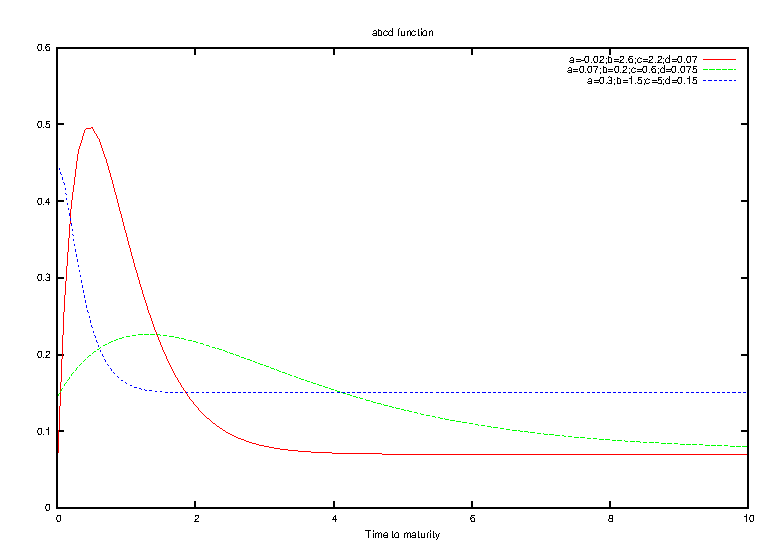
\includegraphics[scale=0.4]{gnuplot_abcdFunction}
\end{center}
\caption{\label{fig:abcd_curve} Different humped volatility can be modelled by  abcd function}
\end {figure}
abcd volatility shape, perfect time homogeneity property. Humped shape correspond to market normal condition.
\end{frame}

%%%%%%%%%%%%%%%%%%%%%%%%%%%%%%%%
\begin{frame}
\frametitle{Piecewise volatility}
Downside of parameterization abcd
\begin{itemize}
\item Fewness of parameters
\item To much perfect shape is not realist
\end{itemize}
hgVolatility : Separation $\sigma_{ij} = h_{ij}g_{ij}$
\begin{itemize}
\item $h$ matrix initialized by abcd function
\item $g$ matrix allow flexibility by adding degree of freedom
\item calibration essentially done with $g$ matrix
\end{itemize} 
\end{frame}

%%%%%%%%%%%%%%%%%%%%%%%%%%%%%%%%
\begin{frame}
\frametitle{Link Swaption and Caplet}
Swap measure and ito
\[
\frac{d\Sab(t)}{\Sab(t)} = \sigmaab(t)d\Wab(t)
\hspace{1cm}
[\sigmaab(t)]^2 = \frac{ d<\Sab,\Sab>_t }{[\Sab(t)]^2 }
\]
By considering swap rate as weighted sum of libors
\[
[\sigmaab(t)]^2 = \frac{1}{[\Sab(t)]^2 } \sum_{i,j=\alpha}^{\beta-1} w_i(t)w_j(t) d<L_i,L_j>_t
\hspace{1cm}
w_k(t) = \frac{\sum^{\beta-1}_{k=\alpha} \tau_k P(t,T_{k+1}) }{\Cab(t)}
\]
By replacing dynamic of Libors
\[
[\sigmaab(t)]^2 = \frac{1}{[\Sab(t)]^2 } \sum_{i,j=\alpha}^{\beta-1} w_i(t)w_j(t) L_i(t)L_j(t) \rho_{L_{ij}}(t) \sigma_{L_i}(t) \sigma_{L_j}(t) dt
\]
Rebonato approximation formula
\[
\Ta[\sigma^{BLACK}_{\alpha,\beta}]^2 \approx \frac{1}{[\Sab(0)]^2 } \sum_{i,j=\alpha}^{\beta-1} w_i(0)w_j(0)L_i(0)L_j(0) 
\int_{0}^{\Ta} \rho_{L_{ij}}(t) \sigma_{L_i}(t) \sigma_{L_j}(t) dt
\]
\end{frame}


%%%%%%%%%%%%%%%%%%%%%%%%%%%%%%%%%%%%%%%%%%%%%%%%%%%%%%%%%%%%%%%%
\section{Calibration}
%%%%%%%%%%%%%%%%%%%%%%%%%%%%%%%%
\begin{frame}
\frametitle{Bloomberg Data}
\begin{itemize}
\item Use VCUB ATM Swaption and Rebonato approximation to calibrate 
\item Use ICVS to get the discournt rate curve, then interpolate to have the Init libors 
\item Volatility skew
\[
\textbf{derivative}(skew) = \frac{quote (\textbf{ATM+5bp}) - quote(\textbf{ATM-5bp}) }{\textbf{10bp}}
\]
\item data check consistency : recompute swap rate, compare with strike of ATM VCUB, error max 5\%
\end{itemize}
\end{frame}

%%%%%%%%%%%%%%%%%%%%%%%%%%%%%%%%
\begin{frame}
\frametitle{VCUB and volatility parameters dependency}
\psset{unit=0.7cm}
\begin{center}
\begin{pspicture}(-7,-3)(7,4)
%% Reference for Picture
%\psline[linewidth=0.1pt,linecolor=gray](-7,-3)(7,4)
%\rput(-6,-3){(-6,-3)}\rput(-1,2){(-1,2)}
%\rput(2,-3){(2,-3)}\rput(7,2){(7,2)}\rput(0,0){(0,0)}
%%%%%%%%%%%%%%%%%%%%%%%%%%%%%%%%%%%%%%%%%%%%%%%%%%%%%%%%%%%%%%%%%%%%
%% Draw for Swaption matrix
\psgrid[subgriddiv=1,gridcolor=gray,griddots=10,gridlabels=0](-6,-3)(-1,2)                 % set grid for Swaptions matrix
\rput(-5,2.3){$1^{YR}$}\rput(-4,2.3){$2^{YR}$}\rput(-3,2.3){$3^{YR}$}\rput(-2,2.3){$4^{YR}$}\rput(-1,2.3){$5^{YR}$} % set horizontal label for Swaption matrix
\rput(-6.5,1){$1_{YR}$}\rput(-6.5,0){$2_{YR}$}\rput(-6.5,-1){$3_{YR}$}\rput(-6.5,-2){$4_{YR}$}\rput(-6.5,-3){$5_{YR}$} % set vertibal label for Swaption matrix
\psset{linecolor=red} % set points for swaption matrix
%\qdisk(-5,1){3pt}\qdisk(-4,1){3pt}\qdisk(-3,1){3pt}\qdisk(-2,1){3pt}
%\qdisk(-5,0){3pt}\qdisk(-4,0){3pt}\qdisk(-3,0){3pt}
%\qdisk(-5,-1){3pt}\qdisk(-4,-1){3pt}\qdisk(-5,-2){3pt}
\psdots[dotstyle=*,dotscale=2](-5,1)(-4,1)(-3,1)(-2,1)(-5,0)(-4,0)(-3,0)(-5,-1)(-4,-1)(-5,-2)
\psset{linecolor=black}
\rput(-5.5,3){$\scriptstyle\text{nbSwap} = \frac{1}{2}(\text{nbYR}-1)\text{nbYR}=10 $}
%%%%%% draw the dependance zone for Swaption 3YRx2YR
%\pspolygon[linearc=.2,fillstyle=crosshatch,hatchcolor=gray,hatchwidth=0.1pt,hatchsep=1pt,linestyle=none](-4.5,-0.5)(-3.5,-0.5)(-3.5,-1.5)(-4.5,-1.5)
\pscircle[linearc=.2,fillstyle=crosshatch,hatchcolor=gray,hatchwidth=0.1pt,hatchsep=1pt,linestyle=none](-4,-1){0.5}
%%%%%%%%%%%%%%%%%%%%%%%%%%%%%%%%%%%%%%%%%%%%%%%%%%%%%%%%%%%%%%%%%%%%
%% Draw for Vol piece wise matrix
\psgrid[gridwidth=0.01pt,gridcolor=lightgray,subgriddiv=2,subgridwidth=0.1pt,subgridcolor=lightgray,gridlabels=0](2,-3)(7,2)          % set grid for vol matrix
%% set horizon label for vol matrix
\rput(2,2.1){$\scriptstyle{T_0}$}\rput(2.5,2.1){$\scriptstyle{T_1}$}
\rput(3,2.1){$\scriptstyle{T_2}$}\rput(3.5,2.1){$\scriptstyle{T_3}$}
\rput(4,2.1){$\scriptstyle{T_4}$}\rput(4.5,2.1){$\scriptstyle{T_5}$}
\rput(5,2.1){$\scriptstyle{T_6}$}\rput(5.5,2.1){$\scriptstyle{T_7}$}
\rput(6,2.1){$\scriptstyle{T_8}$}\rput(6.5,2.1){$\scriptstyle{T_9}$}
\rput(7,2.1){$\scriptstyle{T_{10}}$} 
%% set vertical label for vol matrix
\rput(1.5,1){$g_2(t)$}\rput(1.5,0){$g_4(t)$}\rput(1.5,-1){$g_6(t)$}\rput(1.5,-2){$g_8(t)$}\rput(1.5,-3){$g_{10}(t)$}     
%%
%%%%%% set points for calibrating vol
{%%
\psset{linecolor=blue} 
\psdots[dotstyle=square*,dotscale=1.5](3,0.5)(3,-0.5)(4,-0.5)(3,-1.5)(4,-1.5)(5,-1.5)(3,-2.5)(4,-2.5)(5,-2.5)(6,-2.5)
}%%
%%%%%% draw line for piecewise constant vol points
\psset{linewidth=1.2pt}
\qline(2.5,1.5)(2.1,1.5) %
\qline(2.5,1)(2.1,1)\qline(3,1)(2.6,1) %
\qline(2.5,0.5)(2.1,0.5)\qline(3,0.5)(2.6,0.5)\qline(3.5,0.5)(3.1,0.5) %
\qline(2.5,0)(2.1,0)\qline(3,0)(2.6,0)\qline(3.5,0)(3.1,0)\qline(4,0)(3.6,0) %
\qline(2.5,-0.5)(2.1,-0.5)\qline(3,-0.5)(2.6,-0.5)\qline(3.5,-0.5)(3.1,-0.5)\qline(4,-0.5)(3.6,-0.5)\qline(4.5,-0.5)(4.1,-0.5) %
\qline(2.5,-1)(2.1,-1)\qline(3,-1)(2.6,-1)\qline(3.5,-1)(3.1,-1)\qline(4,-1)(3.6,-1)\qline(4.5,-1)(4.1,-1)\qline(5,-1)(4.6,-1) %
\qline(2.5,-1.5)(2.1,-1.5)\qline(3,-1.5)(2.6,-1.5)\qline(3.5,-1.5)(3.1,-1.5)\qline(4,-1.5)(3.6,-1.5)\qline(4.5,-1.5)(4.1,-1.5)\qline(5,-1.5)(4.6,-1.5)\qline(5.5,-1.5)(5.1,-1.5) %
\qline(2.5,-2)(2.1,-2)\qline(3,-2)(2.6,-2)\qline(3.5,-2)(3.1,-2)\qline(4,-2)(3.6,-2)\qline(4.5,-2)(4.1,-2)\qline(5,-2)(4.6,-2)\qline(5.5,-2)(5.1,-2)\qline(6,-2)(5.6,-2) %
\qline(2.5,-2.5)(2.1,-2.5)\qline(3,-2.5)(2.6,-2.5)\qline(3.5,-2.5)(3.1,-2.5)\qline(4,-2.5)(3.6,-2.5)\qline(4.5,-2.5)(4.1,-2.5)\qline(5,-2.5)(4.6,-2.5)\qline(5.5,-2.5)(5.1,-2.5)\qline(6,-2.5)(5.6,-2.5)\qline(6.5,-2.5)(6.1,-2.5) %
\qline(2.5,-3)(2.1,-3)\qline(3,-3)(2.6,-3)\qline(3.5,-3)(3.1,-3)\qline(4,-3)(3.6,-3)\qline(4.5,-3)(4.1,-3)\qline(5,-3)(4.6,-3)\qline(5.5,-3)(5.1,-3)\qline(6,-3)(5.6,-3)\qline(6.5,-3)(6.1,-3)\qline(7,-3)(6.6,-3) %
%%%%%% draw line for piecewise constant vol points
\rput(5.5,3){$\scriptstyle\text{nbParam} = \frac{1}{2}(\text{nbLBR}-1)\text{nbLBR}=55 $}
%%%%%% draw the dependance zone for Swaption 3YRx2YR
{
\pspolygon[linearc=.2,fillstyle=crosshatch,hatchcolor=gray,hatchwidth=0.1pt,hatchsep=1pt,linestyle=none](2.35,-0.85)(5.15,-0.85)(5.15,-2.65)(2.35,-2.65)
}
\end{pspicture}
\end{center}
\end{frame}


%%%%%%%%%%%%%%%%%%%%%%%%%%%%%%%%
\begin{frame}
\frametitle{Interpolation-Extrapolation gMatrix}
Interpolation, Extrapolation zone, cascade idea
\begin{figure}[h]
\psset{unit=0.7cm}
\begin{center}
\begin{pspicture}(-7,-3)(7,3)
%% Reference for Picture
%\psline[linewidth=0.1pt,linecolor=gray](-7,-3)(7,3)
%\rput(-6,-3){(-6,-3)}\rput(-1,2){(-1,2)}\rput(2,-3){(2,-3)}\rput(7,2){(7,2)}\rput(0,0){(0,0)}
%%%%%%%%%%%%%%%%%%%%%%%%%%%%%%%%%%%%%%%%%%%%%%%%%%%%%%%%
%% Draw for Global Calibrate and Interpolate
\psgrid[gridwidth=0.01pt,gridcolor=lightgray,subgriddiv=2,subgridwidth=0.01pt,subgridcolor=lightgray,gridlabels=0](-6,-3)(-1,2)          % set grid for vol matrix
%% set horizon label for vol matrix
\rput(-6,2.1){$\scriptstyle{T_0}$}\rput(-5.5,2.1){$\scriptstyle{T_1}$}
\rput(-5,2.1){$\scriptstyle{T_2}$}\rput(-4.5,2.1){$\scriptstyle{T_3}$}
\rput(-4,2.1){$\scriptstyle{T_4}$}\rput(-3.5,2.1){$\scriptstyle{T_5}$}
\rput(-3,2.1){$\scriptstyle{T_6}$}\rput(-2.5,2.1){$\scriptstyle{T_7}$}
\rput(-2,2.1){$\scriptstyle{T_8}$}\rput(-1.5,2.1){$\scriptstyle{T_9}$}
\rput(-1,2.1){$\scriptstyle{T_{10}}$} 
%%
%%%%%%% set points for calibrating vol
{\psset{linecolor=blue} 
\psdots[dotstyle=square*,dotscale=1.5](-5,0.5)(-5,-0.5)(-4,-0.5)(-5,-1.5)(-4,-1.5)(-3,-1.5)(-5,-2.5)(-4,-2.5)(-3,-2.5)(-2,-2.5)
}%%%%%%
%%
%%%%%%% set interpolated points
{\psset{dotsize=3pt} 
\psdots[dotstyle=pentagon*](-5,0)(-5,-1)(-5,-2)
\psdots[dotstyle=pentagon*](-4.5,0)(-4.5,-0.5)(-4.5,-1)(-4.5,-1.5)(-4.5,-2)(-4.5,-2.5)
\psdots[dotstyle=pentagon*](-4,-1)(-4,-2)
\psdots[dotstyle=pentagon*](-3.5,-1)(-3.5,-1.5)(-3.5,-2)(-3.5,-2.5)
\psdots[dotstyle=pentagon*](-3,-2)(-2.5,-2)(-2.5,-2.5)
}%%%%%%
%%
%% set the interpolation zone
\pspolygon[fillstyle=crosshatch,hatchcolor=gray,hatchwidth=0.01pt,hatchsep=1pt,linestyle=none](-5,0.5)(-5,-2.5)(-2,-2.5)
%%
%% set the extrapolate zone
\pspolygon[fillstyle=crosshatch,hatchcolor=gray,hatchwidth=0.01pt,hatchsep=4pt,hatchangle=20,linestyle=none](-5.5,1.5)(-1,-3)(-5.5,-3)
%%
%% Set extrapolation arrows
{%%%%
\psset{linewidth=0.1pt}
\psline{->}(-5,0.5)(-5.5,1.5)\psline{->}(-5,0.5)(-5.5,1)\psline{->}(-5,0.5)(-5.5,0.5)\psline{->}(-5,0.5)(-4.5,0.5)
\psline{->}(-5,0)(-5.5,0)\psline{->}(-4.5,0)(-4,0)
\psline{->}(-5,-0.5)(-5.5,-0.5)\psline{->}(-4,-0.5)(-3.5,-0.5)
\psline{->}(-5,-1)(-5.5,-1)\psline{->}(-3.5,-1)(-3,-1)
\psline{->}(-5,-1.5)(-5.5,-1.5)\psline{->}(-3,-1.5)(-2.5,-1.5)
\psline{->}(-5,-2)(-5.5,-2)\psline{->}(-2.5,-2)(-2,-2)
\psline{->}(-5,-2.5)(-5.5,-2.5)\psline{->}(-2,-2.5)(-1.5,-2.5)
\psline{->}(-5,-2.5)(-5.5,-3)
\psline{->}(-5,-2.5)(-5,-3)
\psline{->}(-4.5,-2.5)(-4.5,-3)
\psline{->}(-4,-2.5)(-4,-3)
\psline{->}(-3.5,-2.5)(-3.5,-3)
\psline{->}(-3,-2.5)(-3,-3)
\psline{->}(-2.5,-2.5)(-2.5,-3)
\psline{->}(-2,-2.5)(-2,-3)
\psline{->}(-2,-2.5)(-1,-3)
}%%%% Set extrapolation arrows
%%%%%%%%%%%%%%%%%%%%%%%%%%%%%%%%%%%%%%%%%%%%%%%%%%%%%%%%
%% Draw for local Calibrate and Interpolate
\psgrid[gridwidth=0.01pt,gridcolor=lightgray,subgriddiv=2,subgridwidth=0.01pt,subgridcolor=lightgray,gridlabels=0](2,-3)(7,2)          % set grid for vol matrix
%%
%% set horizon label for vol matrix
\rput(2,2.1){$\scriptstyle{T_0}$}\rput(2.5,2.1){$\scriptstyle{T_1}$}
\rput(3,2.1){$\scriptstyle{T_2}$}\rput(3.5,2.1){$\scriptstyle{T_3}$}
\rput(4,2.1){$\scriptstyle{T_4}$}\rput(4.5,2.1){$\scriptstyle{T_5}$}
\rput(5,2.1){$\scriptstyle{T_6}$}\rput(5.5,2.1){$\scriptstyle{T_7}$}
\rput(6,2.1){$\scriptstyle{T_8}$}\rput(6.5,2.1){$\scriptstyle{T_9}$}
\rput(7,2.1){$\scriptstyle{T_{10}}$} 
%%
%% set points for calibrating vol
{%%%%
\psset{linecolor=blue} 
\psdots[dotstyle=square*,dotscale=1.5](4,-0.5)(4,-1.5)(4,-2.5)
}%%%% set points for calibrating vol
%%
%%%%%%% set interpolated points
{\psset{dotsize=3pt} 
\psdots[dotstyle=pentagon*](3.5,0)(3.5,-0.5)(3.5,-1)(3.5,-1.5)(3.5,-2)(3.5,-2.5)
\psdots[dotstyle=pentagon*](4,-1)(4,-2)
}%%%%%%
%%
%% set the interpolation zone
\pspolygon[fillstyle=crosshatch,hatchcolor=gray,hatchwidth=0.01pt,hatchsep=1pt,linestyle=none](3,0.5)(4,-0.5)(4,-2.5)(3,-2.5)
%%
%% set the extrapolate zone
\pspolygon[fillstyle=crosshatch,hatchcolor=gray,hatchwidth=0.03pt,hatchsep=3pt,hatchangle=30,linestyle=none](2.5,1.5)(4,0)(4,-3)(2.5,-3)
%%
%% Set extrapolation arrows
{%%%%
\psset{linewidth=0.1pt}
\psline{->}(3.5,0)(4,0)
\psline{->}(3.5,-2.5)(3.5,-3)\psline{->}(4,-2.5)(4,-3)
}%%%% Set extrapolation arrows
\end{pspicture}
\end{center}
\caption{\label{fig:interpolation_matrix} Interpolation and Extrapolation for volatility matrix}
\end{figure}
\end{frame}

%%%%%%%%%%%%%%%%%%%%%%%%%%%%%%%%
\begin{frame}
\frametitle{G Matrix Mapping}
\begin{figure}[h]
  \centering
  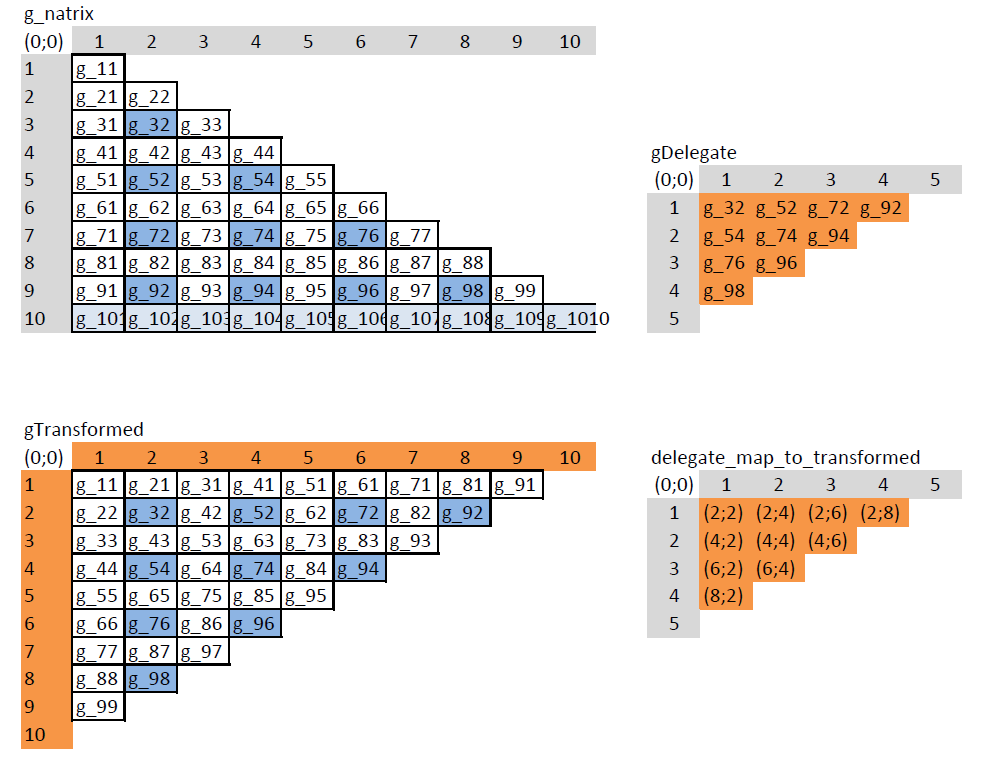
\includegraphics[scale=0.3]{matrix_mapping}
  \caption{\label{fig:matrix_mapping} Matrix Mapping}
\end{figure}
\end{frame}


%%%%%%%%%%%%%%%%%%%%%%%%%%%%%%%%
\begin{frame}
\frametitle{calibration pipeline}
\begin{figure}[h]
\begin{center}
\begin{pspicture}(-6,-2)(6,2)
\psset{unit=0.8cm}
\tiny
%% Reference for Picture
%\psline[linewidth=0.1pt,linecolor=gray](-6,-2)(6,2) \rput(-6,-2){(-6,-2)}\rput(0,0){(0,0)}\rput(6,2){(6,2)}
%%%%%%
\rput(-5,0){\rnode{gD}{\psframebox{gDelegate} }}
\rput(-3,2){\rnode{gT}{\psframebox{gTransfomed} }}
\rput(-2,0){\rnode{g}{\psframebox{gMatrix} }}
\rput(3.5,0){\rnode{MDL}{\psframebox{MDL Quote} }}
\rput(3.5,-1.5){\rnode{MKT}{\psframebox{MKT Quote} }}
\rput(1.5,-0.8){\rnode{diff}{\psframebox{Diff} }}
\nccurve[angleA=60,angleB=-110]{->}{gD}{gT}
\nccurve[angleA=-70,angleB=110]{->}{gT}{g}
\nccurve[angleB=180]{->}{g}{MDL}\rput(0.8,0.2){Rebonato Approx}
\nccurve[angleA=-90]{->}{MDL}{diff}
\nccurve[angleA=90]{->}{MKT}{diff}
\nccurve[angleA=200,angleB=-90]{->}{diff}{gD}\rput(-2.5,-2.){\tiny Minimizer $||\text{\tiny Rebonato(gDelegate)} - \text{\tiny MKT Quotes}||^2$ }
\end{pspicture}
\end{center}
\caption{\label{fig:calibration_pipeline} Calibration Pipeline}
\end{figure}
\end{frame}

%%%%%%%%%%%%%%%%%%%%%%%%%%%%%%%%
\begin{frame}
\frametitle{Regularization - general view}
Cost Function with penalties
\[
	\textbf{Cost Function} = (\textbf{MDL Quote} - \textbf{MKT Quote}) + \text{Pel}_{T} + \text{Pel}_{M}
\]
\begin{columns}[t]
\column{.5\textwidth}
\centering
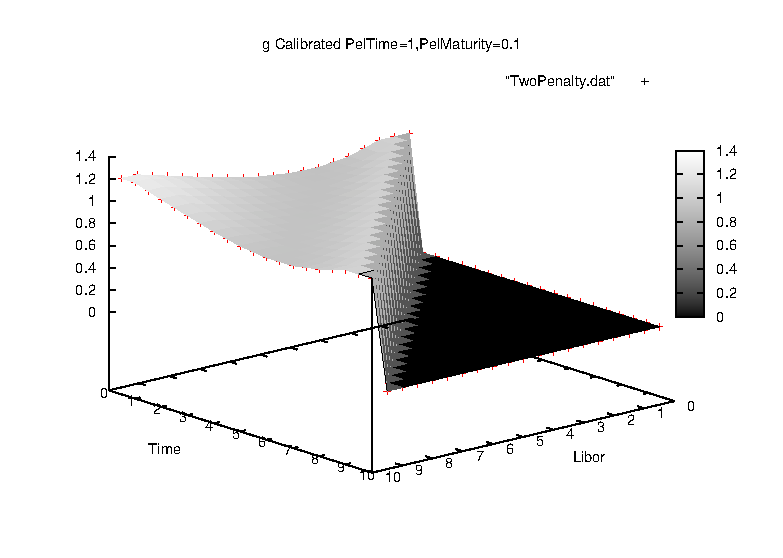
\includegraphics[width=5cm,height=3.5cm]{PenaltyTwo}
\column{.5\textwidth}
\centering
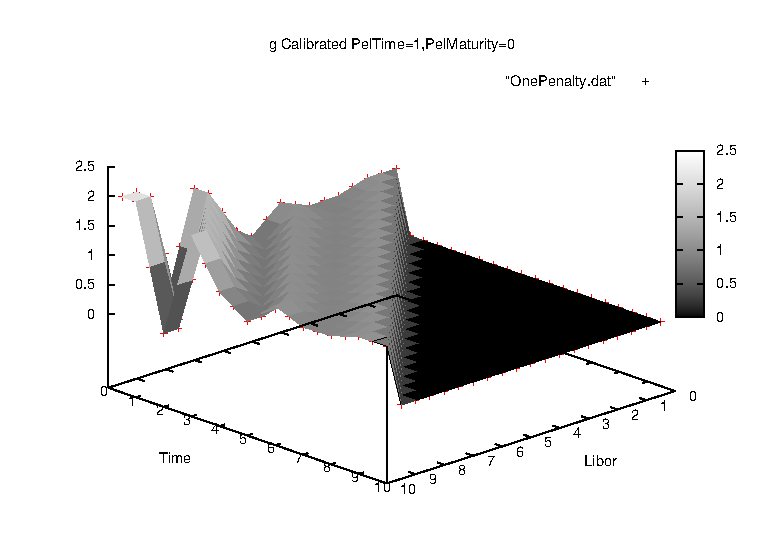
\includegraphics[width=5cm,height=4cm]{PenaltyOne}
\end{columns}
\end{frame}

%%%%%%%%%%%%%%%%%%%%%%%%%%%%%%%%
\begin{frame}
\frametitle{Regularization - Time Homogeneuous Penalty}
Wish time homogeneity for $g$
\[
g(t,T) = \Phi(T-t) = \Phi(\tau)   \hspace{2cm} \forall 0 \leq t \leq T \hspace{0.5cm} \tau = T-t
\]
Penalty on $g$
\[
 |\frac{\partial g}{\partial \tau}(t,T) | < \text{Const} \hspace{2cm} \tau = T-t
\]
computation on gDelegate
\[
\text{Pel}_{T} = \textbf{c}_{T}(\sum_j \sum_i \text{gDelegate}_{(i+1,j)} - \text{gDelegate}_{(i,j)} )
\]
\end{frame}

%%%%%%%%%%%%%%%%%%%%%%%%%%%%%%%%
\begin{frame}
\frametitle{Regularization - Maturity Smoothness Penalty}
Penalty on $g$
\[
 |\frac{\partial^2 g}{\partial T^2}(t,T) | < \text{Const}
\]
Computation
\[
\text{Pel}_{M} = \textbf{c}_{M} (\sum_i \sum_j \text{gDelegate}_{(i,j-1)} + \text{gDelegate}_{(i,j+1)} - 2 \text{gDelegate}_{(i,j)} )
\]
\end{frame}

%%%%%%%%%%%%%%%%%%%%%%%%%%%%%%%%%%%%%%%%%%%%%%%%%%%%%%%%%%%%%%%%
\section{Virtual Test and numerical results}

%%%%%%%%%%%%%%%%%%%%%%%%%%%%%%%%
\begin{frame}
\frametitle{Virtual test pipeline}
Seed , Noises
\begin{figure}[h]
\begin{center}
\begin{pspicture}(-6,-2)(6,2)
%% Reference for Picture
%\psline[linewidth=0.1pt,linecolor=gray](-6,-2)(6,2)
\rput(-5,0){\rnode{TP}{\psframebox{True Param} }}
\rput(-1,2){\rnode{MK}{\psframebox[framearc=0.4]{VIRTUAL MKT DATA} }}
\rput(1,0){\ovalnode{C}{Calibrator} }
\rput(2,-2){\rnode{PP}{\psframebox[framearc=0.4]{Perturbed Param} }}
\nccurve[angleA=90,angleB=180]{->}{TP}{MK}
\nccurve[angleA=-90,angleB=180]{->}{TP}{PP}
\nccurve[angleB=10]{->}{MK}{C}
\nccurve[angleA=90,angleB=-10]{->}{PP}{C}
\ncline[nodesep=3pt]{->}{C}{TP}
\rput(-4.6,-0.5){\tiny seed}
\end{pspicture}
\end{center}
\caption{\label{fig:virtual_test} Virtual Test Pipeline}
\end{figure}
\end{frame}

%%%%%%%%%%%%%%%%%%%%%%%%%%%%%%%%
\begin{frame}
\frametitle{Results of Exact Virtual Calibration test}
\begin{columns}[t]
\column{.5\textwidth}
\centering
\begin{itemize}
\item noise perturb 50\%, "true" %g% noised 20\% 
\item test with different seeds
\item test with 3 calibrators
\item error around zero
\item time growth
\end{itemize}
\column{.5\textwidth}
\centering
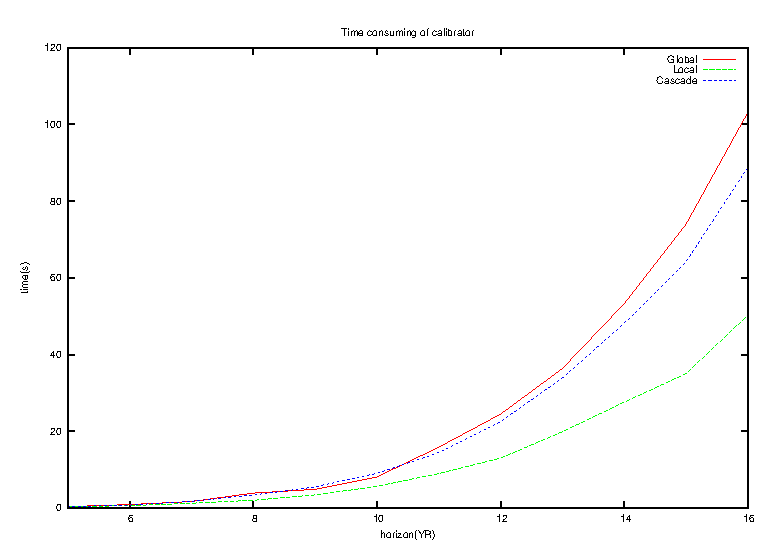
\includegraphics[scale=0.4]{CalibratorTime}
\end{columns}
\end{frame}

%%%%%%%%%%%%%%%%%%%%%%%%%%%%%%%%
\begin{frame}
\frametitle{Results of Regularized Virtual Calibration test}
\begin{columns}[t]
\column{.5\textwidth}
\centering
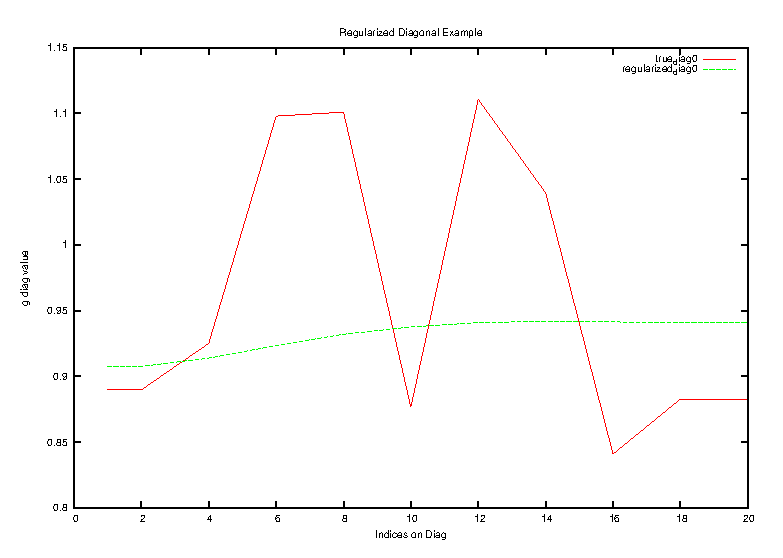
\includegraphics[width=5cm,height=3.5cm]{diag_compare} \\
Regularized diagonal result
\column{.5\textwidth}
\centering
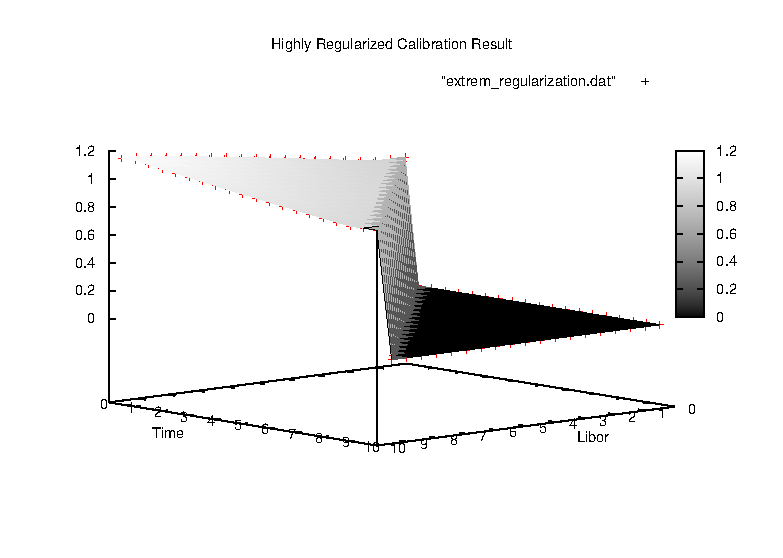
\includegraphics[width=5cm,height=4cm]{extrem_regularization}\\
Highly regularized result
\end{columns}
\end{frame}


%%%%%%%%%%%%%%%%%%%%%%%%%%%%%%%%
\begin{frame}
\frametitle{Analysis error variation in penalties coeff choices}
\begin{columns}[t]
\column{.5\textwidth}
\centering
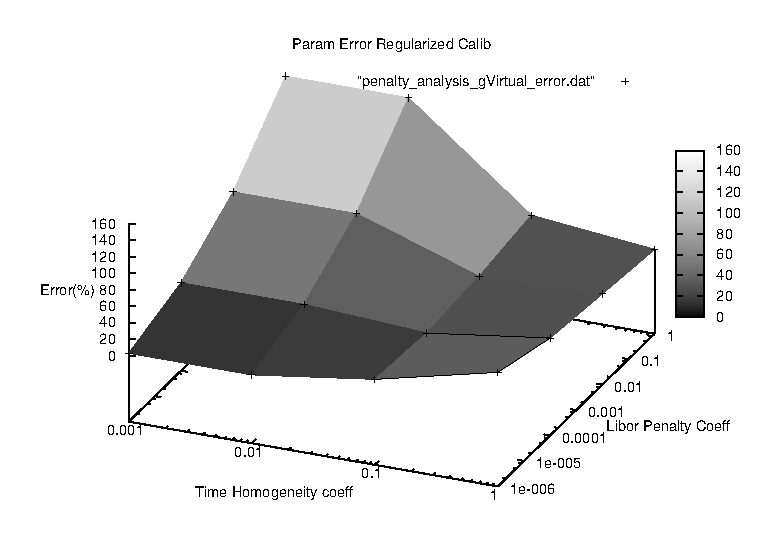
\includegraphics[width=5cm,height=3.5cm]{penalty_analysis_gVirtual_error} \\
Error of param
\column{.5\textwidth}
\centering
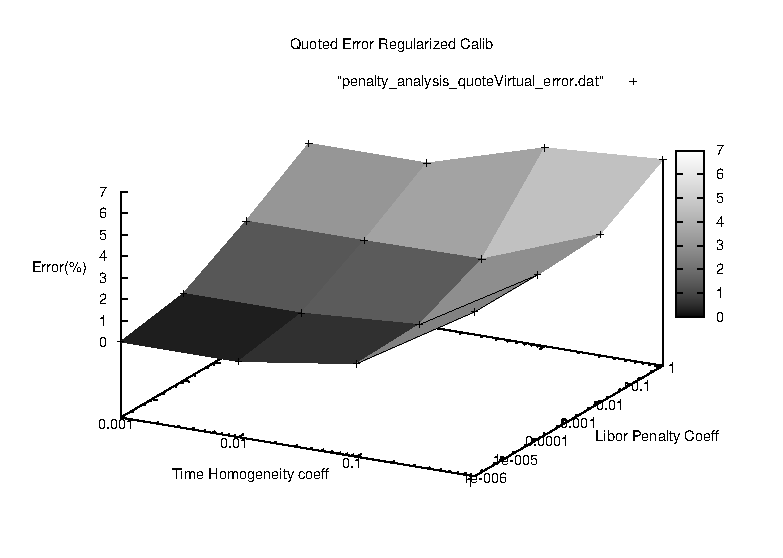
\includegraphics[width=5cm,height=4cm]{penalty_analysis_quoteVirtual_error}\\
Error of Quotation
\end{columns}
\end{frame}

%%%%%%%%%%%%%%%%%%%%%%%%%%%%%%%%
\begin{frame}
\frametitle{Real Data calibration 01-Aug-2014}
\begin{columns}[t]
\column{.5\textwidth}
\centering
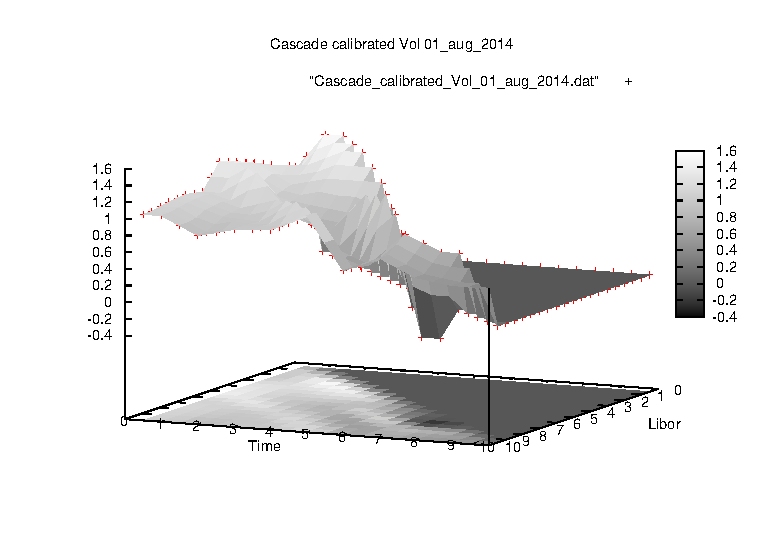
\includegraphics[width=5cm,height=3.5cm]{Cascade_calibrated_Vol_01_aug_2014} \\
Cascade Calibration as analysis tool
\column{.5\textwidth}
\centering
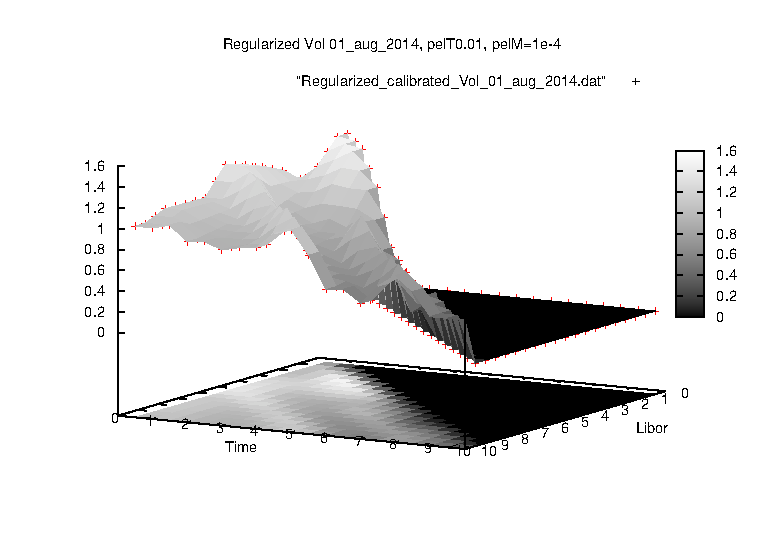
\includegraphics[width=5cm,height=4cm]{Regularized_calibrated_Vol_01_aug_2014}\\
Regularized Calibration
\end{columns}
\end{frame}




%%%%%%%%%%%%%%%%%%%%%%%%%%%%%%%%
\begin{frame}
\frametitle{End}
\begin{center}
Thank you! any Question?
\end{center}

\end{frame}



\end{document}
